\begin{tikzpicture}
\begin{axis}[
    xlabel = $x$,
    ylabel = $y$,
    ymin = -10,
    ymax = 10
]

\addplot[mark=none, smooth, domain = -2:2] {x^2};
\addlegendentry{$y=x^2$};

\only<3->{
\addplot[mark=none, red, smooth, domain = -2:2] {x^3};
\addlegendentry{$y=x^3$};}

\only<4->{
\addplot[mark=none, green, smooth, domain = -2:2] {x^4};
\addlegendentry{$y=x^4$};
}

\only<5->{
\addplot[mark=none, blue, smooth, domain = -2:2] {x^5};
\addlegendentry{$y=x^5$};
}



\end{axis}
\end{tikzpicture}

